% Authors:
% [FB] Filip Bartek
% [BT] Bojana Todorović

% Deadline: Monday 2014-06-16 23:55

% Course page (Ucilnica):
% https://ucilnica.fri.uni-lj.si/course/view.php?id=258

% Submission form (Ucilnica):
% https://ucilnica.fri.uni-lj.si/mod/assign/view.php?id=28803

% Article format:
% EAI Endorsed Transactions on Creative Technologies
% http://eai.eu/transaction/creative-technologies
% Short papers: typically 5 (+/- 2) pages (brave new ideas, artistic installations with technological content, technical creative demonstrators).

% LaTeX template:
% ICST Transactions
% http://doc.eai.eu/publications/transactions/latex/

% Help with writing:
% Writing your article
% http://journalauthors.tandf.co.uk/preparation/writing.asp

% [FB] If you get `pdfTeX error (ext4)`, add `draft` option temporarily.
\documentclass[fonts]{icst}
%\documentclass[fonts,draft]{icst}

\usepackage[utf8]{inputenc}
\usepackage[T1]{fontenc}
\usepackage[english]{babel}

\usepackage{csquotes}
\usepackage[official]{eurosym}
\usepackage{graphicx}
\usepackage{rotating}
\usepackage{tabularx}

\bibliographystyle{icstnum}

\newcommand{\slinkyconductor}{\emph{Slinky conductor}}
\newcommand{\slnkcctr}{\texttt{slnkcctr}}

% http://stackoverflow.com/a/2739710
% http://ctan.mirrorcatalogs.com/macros/latex/contrib/pdfpages/pdfpages.pdf
%\usepackage{pdfpages}

% [FB] `hyperref` should be the last `usepackage` in preamble
% [FB] Watch out: may cause trouble when citation overflows a page.
\usepackage[breaklinks,colorlinks,bookmarksopen,bookmarksnumbered,linkcolor=ICSTblue,citecolor=ICSTblue,urlcolor=ICSTblue]{hyperref}

% http://ctan.mirrorcatalogs.com/macros/latex/contrib/breakurl/breakurl.pdf
% At the preamble, just put \usepackage{breakurl} somewhere after
% \usepackage{hyperref}.
\usepackage{breakurl}

% http://en.wikibooks.org/wiki/LaTeX/Glossary
% Any links in resulting glossary will not be "clickable" unless you load the glossaries package after the hyperref package.
% Every time the glossary changes, run `makeglossaries report` in this
% folder.
% http://tex.stackexchange.com/a/46732
\usepackage{glossaries}
\newacronym{ide}{IDE}{integrated development environment}
\newacronym{sfml}{SFML}{Simple and Fast Multimedia Library}
\newacronym{gui}{GUI}{graphical user interface}
\newacronym{api}{API}{application programming interface}
\makeglossaries

\begin{document}

\runningheads {F.~Bártek, B.~Todorović}{Slinky conductor}
\title{Slinky conductor: project report}
\author{Filip Bártek, Bojana Todorović}

\abstract{
This paper introduces the music toy \slinkyconductor{}
and summarizes the development process of a prototype of the toy.
}

\keywords{Slinky, juggling, music, toy, software}

\maketitle

\section{Introduction}
% Author: Filip Bartek

Slinky is a spring-like toy invented by a naval engineer Richard James
between the years 1943 and 1945.\cite{bellis:historyofslinky}
It quickly became popular in the United States and it is still
widely available nowadays (see figure \ref{fig:slinky-original}).
Various unofficial Slinky duplicates can be found in shops
around Slovenia and Czech Republic and various e-shops
(see an example in figure \ref{fig:slinky-magic}).

\begin{figure}
  \centering
  %\includegraphics[height=7cm]{100-Slinky-Image.jpg}
  \includegraphics[width=\linewidth]{100-Slinky-Image.jpg}
  % Source:
  % http://poof-slinky.com/product/3pk-original-metal-slinky/?pcat_id=301
  \caption{Original Metal Slinky (2014)\cite{poof:slinky}}
  \label{fig:slinky-original}
\end{figure}

\begin{figure}
  \centering
  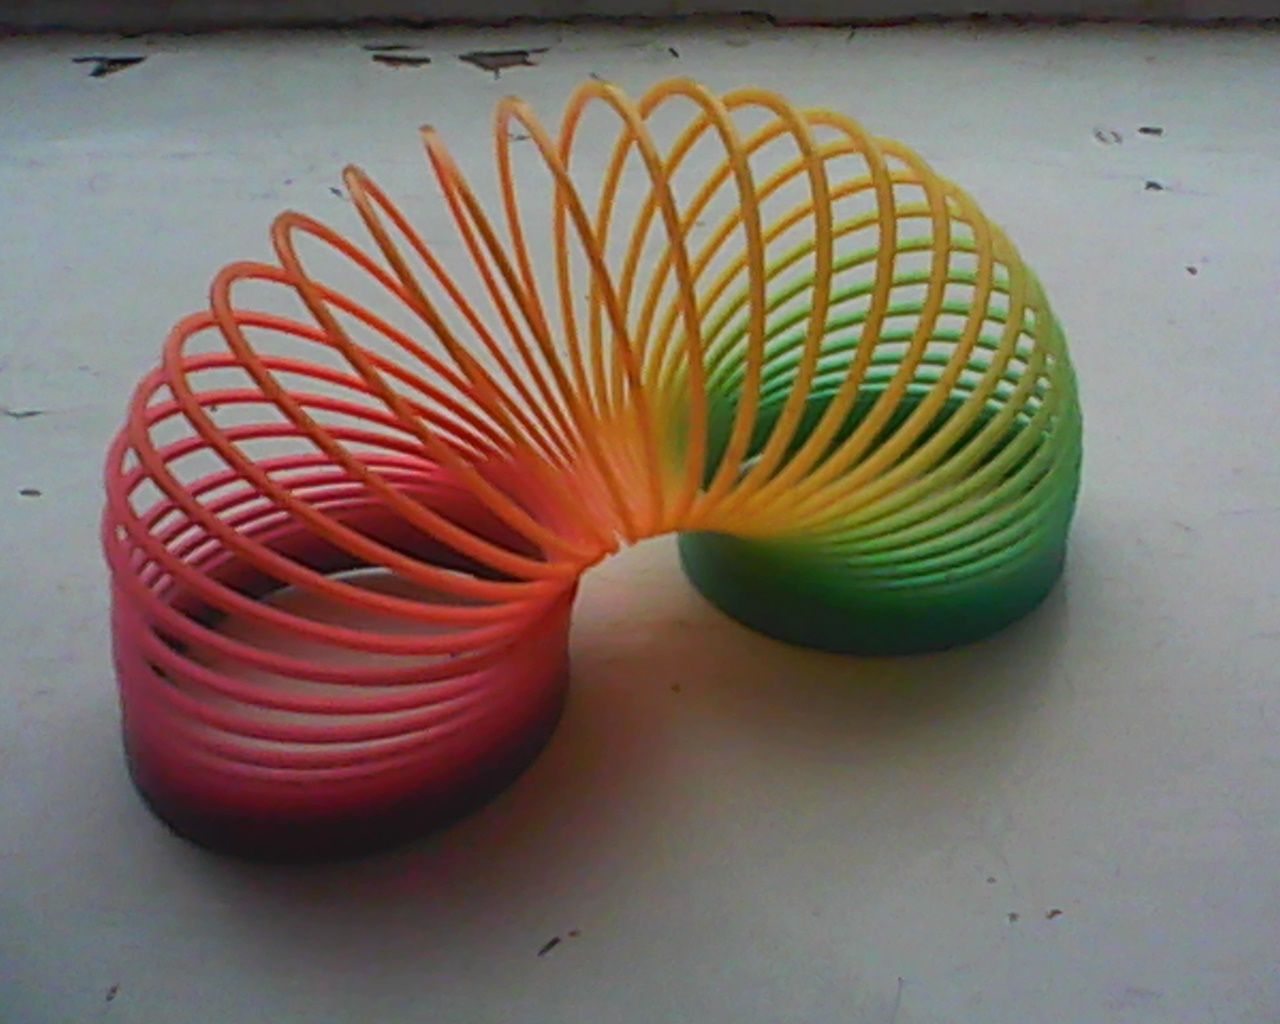
\includegraphics[width=\linewidth]{slinky-magic.jpg}
  \caption{Magic Spring, an unofficial duplicate of the plastic Slinky}
  \label{fig:slinky-magic}
\end{figure}

The physical properties of the toy make it suitable for juggling.
The original manufacturer exposed this potential in
a 1960s TV commercial\cite{youtube:slinky_commercial}
but the overall cultural influence of Slinky juggling
has been extremely limited.

A notable exception
and at the same time a good example of basic Slinky juggling,
which will be referred to as ``slinky walking'' from now on,
can be seen in a video from the \emph{YouTube} user
\emph{tyranicslinky}.\cite{youtube:tyranicslinky}.

\slinkyconductor{} is an imagined software music toy that
plays back music synchronized to a Slinky juggler's performance.

This text describes the development and functionality of
a prototype of \slinkyconductor{}.

In the remainder of the text, we will use the term \emph{slinky}
(with lowercase \emph{s}) as a common name for both
the original Slinky toys and
the unofficial duplicates.
We decided to do so because from the point of view of both
a slinky juggler and
a \slinkyconductor{} user
there is virtually no difference between the two variants of the toy.
However, there \emph{is} significant difference between
metal and plastic slinkys
(see figures \ref{fig:slinky-original} and \ref{fig:slinky-magic}
respectively),
which we will deal with in the next section.
 % text

\section{Project design}

% `\input` in any level

% Author: Filip Bartek

\begin{minipage}{\linewidth}
Project proposal\cite{bartek:proposal} describes the basic desired
behavior of \slinkyconductor{}:

\begin{itemize}
\item when slinky is idle, so is \slinkyconductor{} and
\item when slinky is ``walking'' down the hands of a juggler, \slinkyconductor{} plays back music synchronized to the steps of the slinky.
\end{itemize}
\end{minipage}

We decided to pursue this behavior by implementing
a system that consists of
a computer that runs specialized software (called \slnkcctr{}) and has
a video camera and a sound output device connected to it.
The system (in real-time) tracks the position of slinky
in image from camera,
recognizes the phase in the slinky ``walking'' cycle and
plays back music synchronized to this recognized phase.

% TODO: Make a picture of components here.
% * computer
%     * slnkcctr software
% * camera
% * speakers
% [FB] Suggestion: Use ntikz package.

% TODO: Make a picture of software components here with information
% flow (maybe).
% * slinky position tracker
% * beat recognizer
% * sound player

We decided to use this hardware setup because we feel it's
familiar and affordable for many computer users.
This approach also complements the low-price policy
the original Slinky toy followed throughout most of its history
on behalf of Betty James,
the toy's inventor's wife.\cite[section History]{wiki:slinky}
Indeed, slinky remains a notably affordable toy.\footnote{
As of now,
a package of 3 original Slinkys can be obtained
for \$12.99\cite{poof:slinky}
and the shop \emph{TojeTo} in Ljubljana carries Magic Spring,
a good plastic Slinky duplicate,
for \EUR{2.90}\cite{tojeto:slinky}.
}

For similar reasons, we decided to keep the project
open source\footnote{
The source code of \slnkcctr{} is publicly available
from the \emph{GitHub}
repository \texttt{filiboja/slnkcctr}\cite{filiboja:slnkcctr}.
}
and free to use.

To facilitate visual tracking of the slinky,
we decided to use a brightly colored plastic slinky
instead of the traditional metal variant.
For practical reasons, we further require the slinky to have
different colors at its ends,
and for the colors to be easily separable from background.
We believe that these properties are not uncommon because
most slinkys available around are rainbow-colored
% TODO: Rewrite in a less informal manner.
(see an example in figure \ref{fig:slinky-magic}).
 % text

\subsection{Mind map}

Appendix \ref{app:mindmap} shows project mind map
created in the initial phase of development.

\subsection{Prototype simplification}

We haven't managed to implement
the full proposed functionality\cite{bartek:proposal}
in the prototype presented in this text.
The prototype we have delivered
is able to track the position of a slinky,
determine the approximate timing of slinky steps and
play back simple sounds at the estimated step times.

\section{Implementation}

The operating system Windows was chosen as the target platform
because it's the common platform of the development team.

All the external system components
(see listing in table \ref{tab:systemcomponents})
we used are multi-platform,
so building the software on other platforms remains possible.

Our concern about the performance of real-time slinky tracking process
governed several decisions we made regarding the implementation.

Firstly, we chose to use OpenCV, a computer vision library,
to support visual detection of slinky.
OpenCV is widely used\cite{opencv:about}
and supports many efficient image processing functions
we could use to improve the detection process.

Secondly,
we chose to use C++ as the project's main programming language.
C++ is the main programming language used in OpenCV
and thus we expected the C++ OpenCV \acrshort{api}
to be the most complete and optimized.

% `\input` in a section

% Author: Filip Bartek

\subsection{External software tools}
\subsubsection{System components} \label{sec:systemcomponents}

To facilitate development, we used several existing software libraries
that provide parts of functionality in \slnkcctr{}.
See a list in table \ref{tab:systemcomponents}.

\begin{table}[h]
\centering
\begin{tabularx}{\linewidth}{X|X}
Library & Functionality \\
\hline
\hline
% Breaks just like in `breakurl` package (i.e. after dot and underscore)
% http://ctan.ijs.si/tex-archive/macros/latex/contrib/breakurl/breakurl.pdf
% http://www.boost.org/
Boost.\allowbreak{}Program\_\allowbreak{}options
& Command line ar\-gu\-ments, configuration files \\
\hline
% http://opencv.org/
OpenCV & Object detection, \gls{gui} \\
\hline
% http://www.sfml-dev.org/
\gls{sfml} & Sound playback
\end{tabularx}
\caption{System components}
\label{tab:systemcomponents}
\end{table}

\subsubsection{Development tools}

Throughout the development, we used several stand-alone tools
and one C++ library to deal with various issues.
See a list in table \ref{tab:devtools}.

\begin{table}[h]
\centering
\begin{tabularx}{\linewidth}{X|X}
Tool & Functionality \\
\hline
\hline
% https://github.com/
GitHub & Version control system \\
\hline
Microsoft Visual C++ 2010 Express & C++ \gls{ide} \\
\hline
% https://code.google.com/p/micro-profiler/
MicroProfiler & C++ profiling (library) \\
\hline
% http://avidemux.org/
Avidemux & Video file inspection \\
\hline
% http://www.videolan.org/vlc/
VLC & Media file format conversion \\
\hline
% http://www.dependencywalker.com/
Dependency Walker & Collecting run-time dependencies for a release
\end{tabularx}
\caption{Development tools}
\label{tab:devtools}
\end{table}
 % subsection

% `\input` in a section

% Author: Filip Bartek

\subsection{Architecture}

\slnkcctr{} prototype consists of three main components:

\begin{itemize}
\item slinky end detector,
\item beat detector and
\item sound player.
\end{itemize}

The operation of the components is synchronized with the camera frames.

In each frame and for each of the two ends of the slinky,
a \emph{slinky end detector} tries to detect and localize
the slinky end in the image.

The presence indication and coordinates are then passed to
a \emph{beat detector} which uses this information
and previous values to determine whether
a beat occurred in the current frame.

In case a beat has occurred, \emph{sound player} is asked
to play back a sound corresponding to the slinky end.

% TODO: Optional: Make a picture of components.
 % subsection

% `input` in a section

% Author: Filip Bartek

\subsection{Slinky end detector}
\label{sec:slinkyenddetector}
% http://opencv-srf.blogspot.com/2010/09/object-detection-using-color-seperation.html

Slinky end detection is performed using color filtering.
OpenCV library is used in this step extensively.

The detector takes an image and outputs an estimated position
of an end of slinky in the image.
If slinky end is not detected, a non-position is output.

The detector consists of four filters:

\begin{itemize}
\item \texttt{CropFilter} (crops the image)
\item \texttt{HsvFilter} (filters out some colors)
\item \texttt{OpenFilter} (morphological opening)
\item \texttt{CloseFilter} (morphological closing)
\end{itemize}

The filters select a part of the image, i.e.~a set of pixels.
Slinky end position is determined as the centroid of this set.

Each of the filters is parametrized by one or more numeric values.
The parameters are exposed in \gls{gui} and configuration files.
Refer to the \slnkcctr{} documentation\cite{bartek:slnkcctrreadme}
for details.
 % subsection

% `\input` in a section

% Author: Filip Bartek

\subsection{Beat detector}

Beat detector collects a history (sliding window) of detected
slinky end positions and estimates occurences of steps,
i.e.~moments when the slinky end hits the juggler's hand.

These moments are very easy to determine for a human
observing the juggler
and quite easy to determine for a human reading through a history of
detected slinky end positions,
but implementing a similar functionality in a computer
proved to be quite difficult.

The main factors that contribute to the difficulty
of beat time estimation are:

\begin{itemize}

\item low time resolution of sampled positions
(time resolution is limited by camera frame rate),

\item low precision of sampled positions
(caused by low precision of slinky end detection process,
described in section \ref{sec:slinkyenddetector}) and

\item noise in sampled positions
(caused namely by parts of slinky obscuring the ends while juggling).

\end{itemize}

In the end we resorted to implementing a simple method
optimized for a 15 FPS camera
and a slinky with step period between
$\frac{6}{15}$ and $\frac{12}{15}$ s.
These values were chosen to work with the slinkys and camera
we used for testing
and we believe that
most common slinkys and cameras satisfy these assumptions.

As mentioned above,
the beat detection process proved to be more difficult to implement
than we originally expected
and the current implementation presents a notable room for improvement.
 % subsection

\subsection{Sound player}
% Bojana

For sound playback \slnkcctr{} uses \acrfull{sfml}.

In \slnkcctr{} we used \acrshort{sfml}'s \emph{system module},
which manages the clock and threads,
and \emph{audio module},
which provides an interface to handle sounds and music.

In \slnkcctr{} we implemented a simple beep sound that responds to slinky movement.
The beep sound is a pure sound (i.e.~sine wave) of fixed frequency.

We used two sounds of frequencies 440 and 220 Hz
(to differentiate the slinky ends) and length 0.25 s each.
It is possible to change the frequency, amplitude and length
of the sounds in source code.

\section{Usage}

\slnkcctr{} source code can be obtained
from the GitHub repository\cite{filiboja:slnkcctr}.
Refer to \slnkcctr{} documentation\cite{bartek:slnkcctrreadme}
for setup and usage instructions.

\section{Conclusions}

What makes slinky one of the most popular toys is its simplicity
and the fact that it can perform numerous tricks.

We have implemented a prototype of \slinkyconductor{},
a slinky-controlled music toy.
\slinkyconductor{} is able to support slinky jugglers of all ages
with simple sound effects to accompany their performance.

Potential future development should focus on
improving beat detection precision
and extending the music output with more complex patterns.

\pagebreak

\begin{appendices}

\section{Project mind map}
\label{app:mindmap}
% Bojana

% "include in the written report also an updated mind map of your project!"
% https://ucilnica.fri.uni-lj.si/mod/forum/discuss.php?d=11339

Mind map is a visual representation of important data.
The main concept appears in the centre of the mind map.
Around it there are pieces of relevant information
arranged in intuitively comprehensible patterns.
The pieces of information may be represented by words,
pictures or combinations of both.
Mind map facilitates brainstorming on relevant information
including related work, technology and potential issues.

Figure \ref{fig:mind_map2} shows a \slinkyconductor{} project mind map
conceived early in the development.

\newpage
\begin{sidewaysfigure}
  \centering
  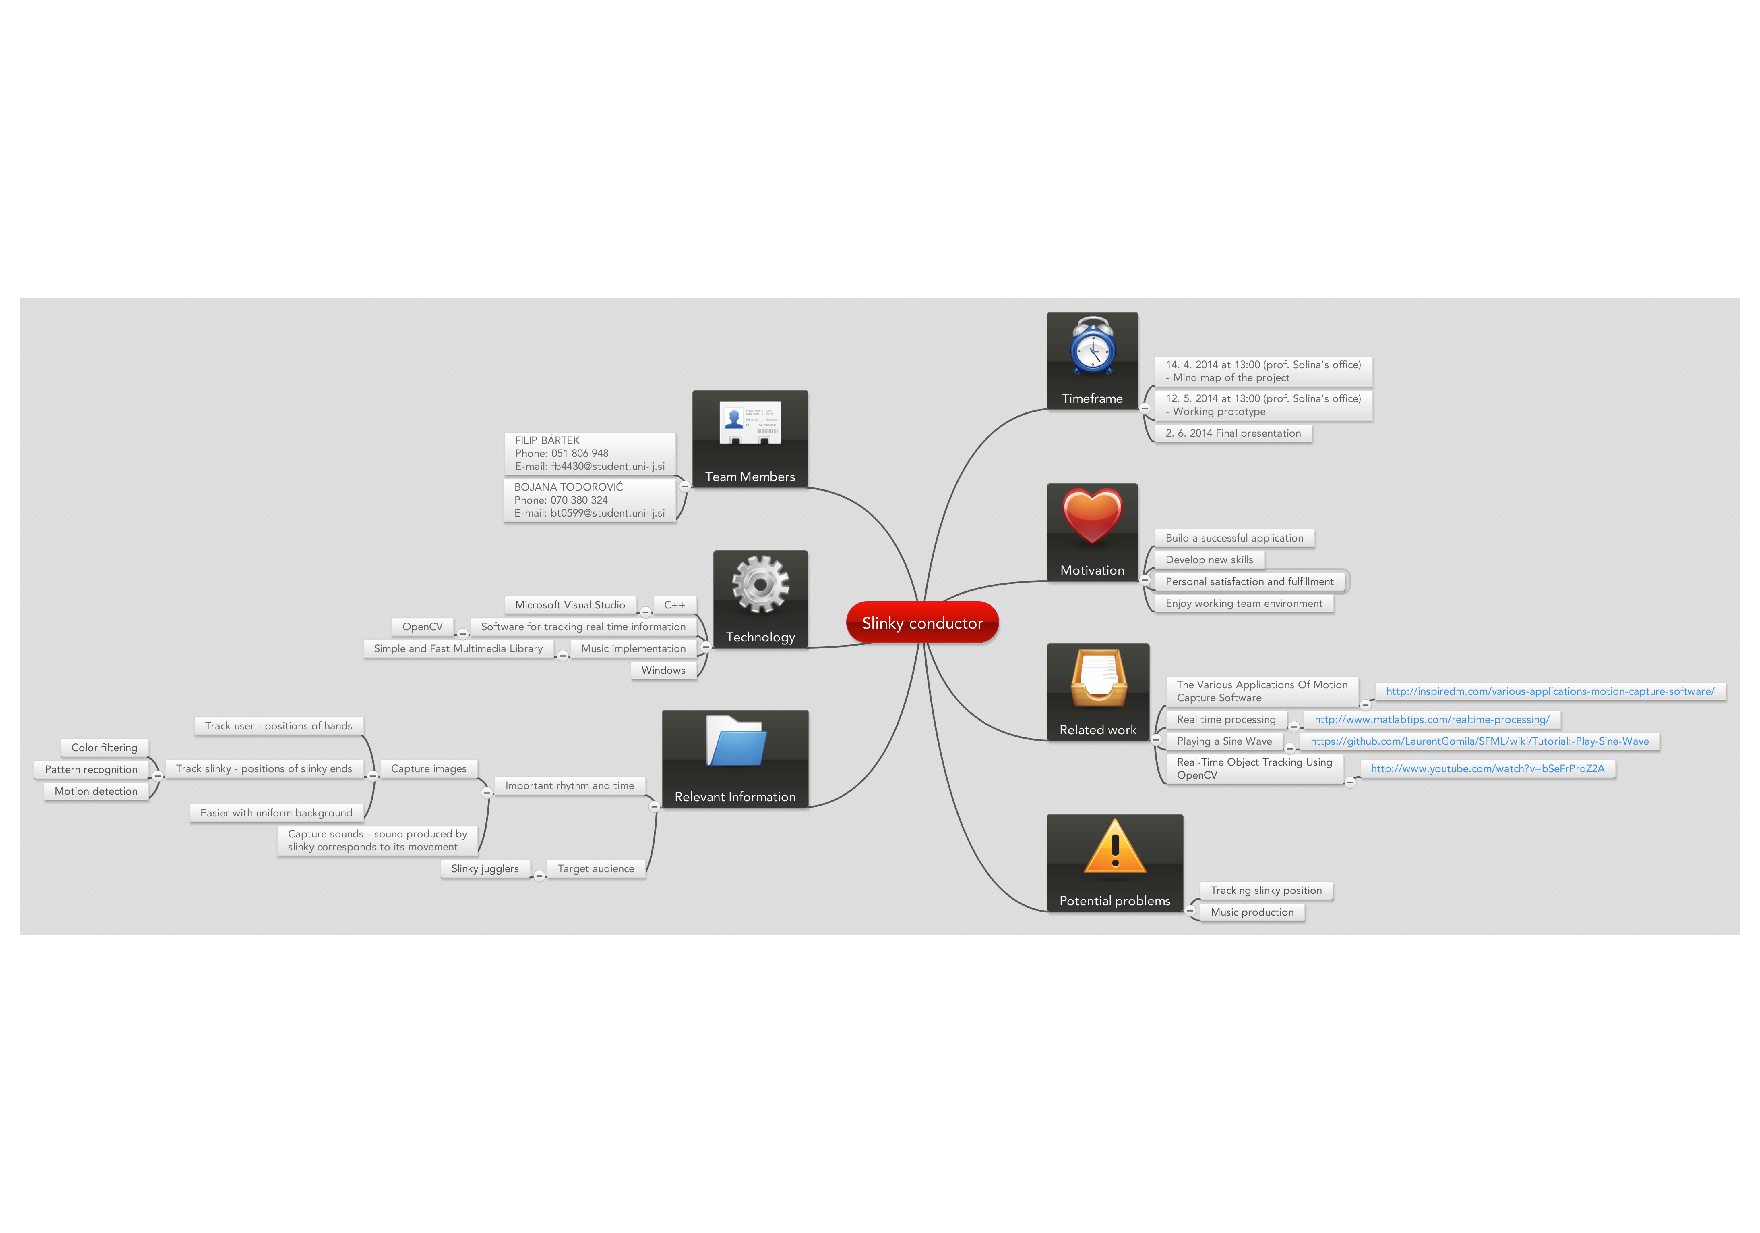
\includegraphics[width=\textheight]{Slinky_conductor.pdf}
  \caption{\slinkyconductor{} mind map}
  \label{fig:mind_map2}
\end{sidewaysfigure}
\newpage

\end{appendices}

\bibliography{report}

\printglossaries{}

\end{document}

%sagemathcloud={"zoom_width":100}